\documentclass{protokol}
\leftheader{Fourierovská infračervená spektroskopie}
% \centerheader{Praktikum IV}
\rightheader{Tomáš Derner}

\begin{document}

  \section*{Úkol}

    \begin{enumerate}
      \item Proměřte rotačně-vibrační absorpční spektrum oxidu uhelnatého ve spektrální oblasti $2000 - \SI{2500}{\per\centi\metre}$. Polohy absorpčních pásů zpracujte graficky a lineární regresí určete parametry vystupující v modelu pružného rotátoru pro základní vibrační stav molekuly a první excitovaný vibrační stav. Z těchto parametrů určete vzdálenosti jader uhlíku a kyslíku v základním a prvním excitovaném vibračním stavu.
      \item Spočtěte teplotní a tlakové rozšíření absorpčních pásů, určete rozdíl vibrační frekvence pro isotopomery \textsuperscript{12}C\textsuperscript{16}O a \textsuperscript{13}C\textsuperscript{16}O. Porovnejte tyto hodnoty s rozlišením použitého spektrálního přístroje.
      \item Změřte spektrum bez vzorku, určete oblasti absorpce oxidu uhličitého a vodních par v optické dráze spektrometru. Interpretujte nejvýraznější pásy absorpce CO\textsubscript{2}.
      \item Proměřte spektra propustnosti polyetylénové a polypropylénové folie a interpretujte nejvýraznější pásy.
      \item Proměřte spektra propustnosti a odrazivosti skleněné a safírové destičky. Diskutujte rozdíl mezi oběma vzorky.
    \end{enumerate}

  \section*{Teorie}

    Cílem této úlohy bylo seznámit se s principy Fourierovské infračervené spektroskopie, konkrétně absorpční vibrační spektroskopie. Nejdůležitější veličinou v infračervené spektroskopii je vlnočet $\nu = \frac{1}{\lambda}$, udávaný v jednotkách $\si{\per\centi\metre}$. Úplnější popis principů infračervené spektroskopie lze nalézt v \cite{pokyny}, zde se omezíme pouze na informace nutné k provedení zadaných výpočtů. V zájmu plynulosti textu bude teorie nutná k popisu naměřených spekter uvedena v sekci výsledků.

    Pro poměr vlnočtů různých dvouatomových molekul je
    \begin{equation}
      \label{eq:isotopomer}
      \frac{\nu_2}{\nu_1} = \sqrt{\frac{\mu_1}{\mu_2}}.
    \end{equation}

    Moment setrvačnosti pro dvouatomovou molekulu otáčející se kolem osy kolmé ke spojnici atomů a procházející těžištěm je 
    \begin{equation} \label{eq:I} 
      I = \mu r_0^2,
    \end{equation}
    kde $\mu$ je redukovaná hmotnost a $r_0$ je vzdálenost atomů.

    Dá se ukázat platnost vztahu pro první excitovaný vibrační stav molekuly CO
    \begin{equation}
      \frac{R_J - P_J}{2 J + 1} = h \left[  (2B_1 - 3D_1) - D_1(2J + 1)^2  \right],
    \end{equation}
    kde $R_J$ je energie přechodu ze stavu s rotačním kvantovým číslem $J$ v pásu R do stavu $J+1$, $P_J$ energie přechodu v pásu P do stavu $J-1$, $h$ je Planckova konstanta a $B_1$ a $D_1$ jsou konstanty, a jeho ekvivalent pro stav základní 
    \begin{equation}
      \frac{R_{J-1} - P_{J+1}}{2J + 1} = h \left[  (2B_0 - 3D_0) - D_0(2J + 1)^2  \right].
    \end{equation}

    Těchto vztahů lze využít k provedení lineární regrese podle předpisu
    \begin{equation}
      \frac{R_J - P_J}{2 J + 1} = - h D_1 (2J + 1)^2 + C_1,
    \end{equation}
    respektive odpovídajícího předpisu pro základní stav. Z této regrese dostaneme hodnotu $D_1$ a $D_0$ a posléze $B_1$ a $B_0$.
    
    Pro konstanty $B$ platí vztah
    \begin{equation}
      B = \frac{h}{8 \pi^2 I},
    \end{equation}    
    ze kterého je možno vyjádřit $I$, dosadit do vzorce \eqref{eq:I} a tak vypočítat vzdálenost atomů v molekule.

    Teplotní rozšíření absorpčních pásů dostaneme ze vztahu
    \begin{equation}
      \delta \nu_T = \frac{\nu_0}{c} \sqrt{\frac{8kT}{m} \ln 2},
    \end{equation}
    kde $\nu_0$ je původní vlnočet, $c \approx \SI{3 e8}{\metre\per\second}$ rychlost světla, $k \approx \SI{1.38 e-23}{\metre\squared\kilogram\per\second\squared\per\kelvin}$ Boltzmannova konstanta, $T$ termodynamická teplota a $m$ hmotnost molekuly.

    Tlakové rozšíření spočteme podle
    \begin{equation}
      \gamma = \left(  \frac{T_{REF}}{T}  \right)^{n_{vzduch}} \left[  \gamma_{vzduch}(p - p_s) + \gamma_s p_s  \right] \approx \gamma_s p,
    \end{equation}
    kde jsme provedli aproximaci $T \approx T_{REF}$, $\gamma_{vzduch} = 0$, $p_s = p$ pro čistý plyn. Hodnota\\ $\gamma_s = \SI{0.1}{\per\centi\metre\per\bar}$.

    
  \section*{Výsledky}

    Měření probíhala s pomocí spektrometru \textit{Vector33} od firmy \textit{Bruker}.

    \subsection*{Úkol 1}

      Pomocí spektrometru při rozlišení $\SI{0.35}{\per\centi\metre}$ bylo proměřeno rotačně-vibrační absorpční spektrum oxidu uhelnatého ve spektrální oblasti $2000 - \SI{2500}{\per\centi\metre}$. Naměřené spektrum přiblížené na oblast obsahující spektrum OH je zobrazeno v grafu v příloze 1.

    \subsection*{Úkol 2}

      Uvažujeme-li $\nu_0 = \SI{2145}{\per\centi\metre}$, $T = \SI{300}{K}$ a $m = 28 \times \SI{1.67 e-27}{kg} = \SI{46.76 e-26}{kg}$, vychází teplotní roztažení absorpčních pásů
      $$ \delta \nu_T \approx \SI{0.0016}{\per\centi\metre}, $$
      což s naším rozlišením nelze naměřit.

      Tlak plynu CO při měření činil $\SI{7}{\milli\bar}$. S touto hodnotou můžeme vypočítat tlakové rozšíření absorpčních pásů
      $$ \gamma \approx \SI{0.7}{\per\centi\metre}. $$ 
      Tato hodnota je rozlišitelná, pásy se tedy nejeví jako bodové.

      Redukovaná hmotnost isotopomeru \textsuperscript{12}C\textsuperscript{16}O je $\mu_{12,16} \doteq \num{6.857}m_n\si{kg}$ a isotopomeru \textsuperscript{13}C\textsuperscript{16}O $ \mu_{13,16} \doteq \num{7.172}m_n\si{kg} $. Uvažujeme-li $\nu_{12,16} = \SI{2145}{\per\centi\metre}$, je podle vztahu \eqref{eq:isotopomer}
      $$ \nu_{13,16} = \SI{2097}{\per\centi\metre}, $$ 
      což je rozlišitelné.

    \subsection*{Úkol 3}

      V příloze 2 je v grafu vyneseno spektrum vzduchu. Měření probíhalo při rozlišení $\SI{0.35}{\per\centi\metre}$ v rozsahu $500 - \SI{4500}{\per\centi\metre}$. 

      V oblasti $1300 - \SI{2000}{\per\centi\metre}$ a $3500 - \SI{4000}{\per\centi\metre}$ můžeme vidět vibrační spektrum vzdušné vlhkosti. V první oblasti je spektrum způsobeno deformačními vibracemi, tedy vibracemi vznikajícími změnou úhlu vodních molekul, v druhé oblasti za spektrum mohou valenční vibrace, tedy ty, při kterých se mění vzdálenost molekul. Vzdálenosti mezi jednotlivými pásy jsou příliš jemné, při použitém rozlišení je v každém binu efektivně integrováno několik pásů. V oblasti kolem $\SI{670}{\per\centi\metre}$ a $\SI{2350}{\per\centi\metre}$ vidíme spektrum CO\textsubscript{2}, přiblížené v grafu \ref{fig:u3}. V oblasti $2260 - \SI{2280}{\per\centi\metre}$ vidíme pravděpodobně jiný isotopomer CO\textsubscript{2}.

      \begin{figure}[H]
        \centering
        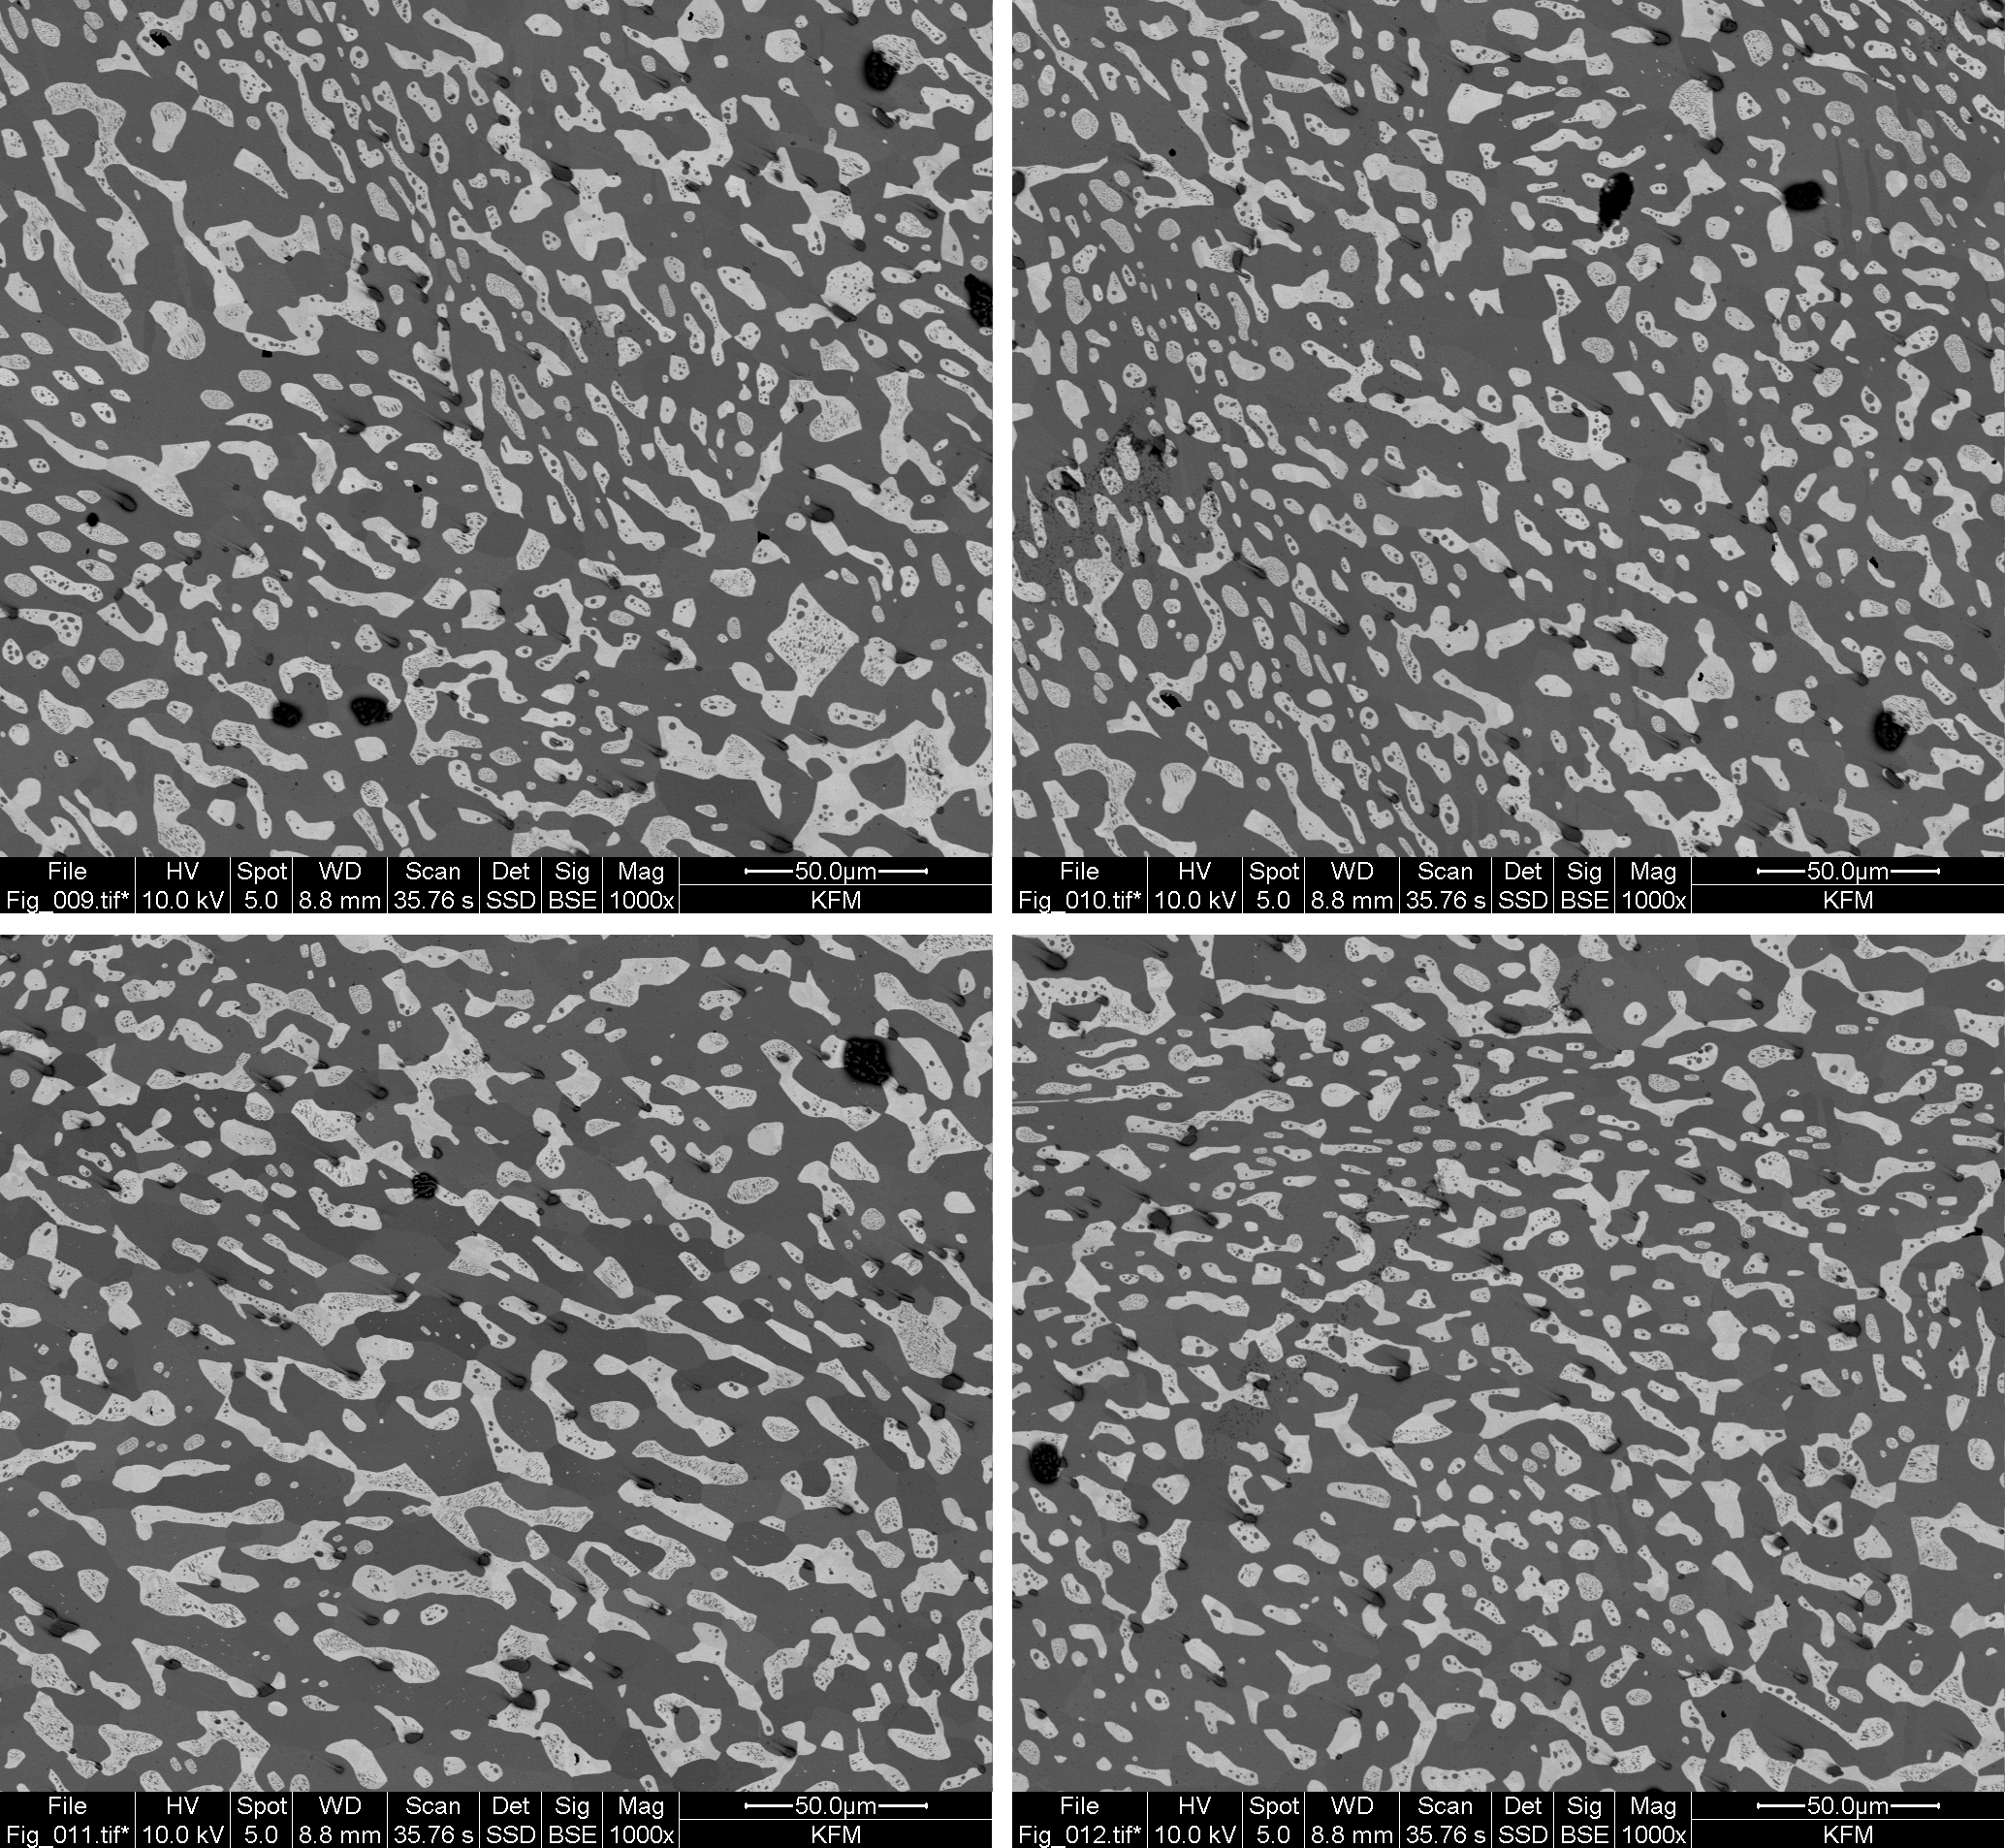
\includegraphics[]{u3}
        \caption{Dvě přiblížení grafu spektra vzduchu (příloha 2)}
        \label{fig:u3}
      \end{figure}

    \subsection*{Úkol 4}
      
      Jako další bylo změřeno spektrum polyetylénové a polypropylénové folie a igelitového sáčku. Měření probíhalo při rozlišení $\SI{2}{\per\centi\metre}$. Grafy lze nalézt v příloze 3. Protože polyetylén má jednodušší strukturu, má zároveň i méně členité spektrum, proto se dá s jistotou říci, že vzorek 1 byla polypropylénová folie, vzorek 2 polyetylénová a igelitový sáček také. Na týchž místech jako ve spektru vzduchu jsou zřejmá spektra vzdušné vlhkosti. V prvním úseku spektra do $\SI{700}{\per\centi\metre}$ je ve spektru vidět interferenční obrazec vznikající interferencí na tenké vrstvě.

    \subsection*{Úkol 5}

      Za použití stejného rozlišení jako v úkolu 4 byly změřeny spektra safírové a skleněné destičky, znázorněné v grafech v příloze 4. Před samotným měřením bylo změřeno spektrum pozadí v odrazu zlatého zrcadla. Kromě opět přítomných spekter vzdušné vlhkosti lze především poukázat na velmi hladký charakter spektra safíru oproti pomaleji a chaotičtěji vzrůstající závislosti transmitance skla. To je dáno pravděpodobně především skutečností, že safírová destička má formu krystalu zatímco sklo je amorfní. Opět je v grafech snadno vidět interferenční obrazec interference na tenké vrstvě.

      Následně se proměřilo odrazové spektrum těchto materiálů, které ukazují grafy v příloze 5. Jak se dá očekávat, mají tato spektra do jisté míry obrácený průběh vůči vůči spektrům předešlým. Kromě opět přítomné vlhkosti a interferenčního obrazce je možné všimnout si, že naměřené spektrum safíru a v menší míře i skla splňuje teoretickou předpověď Drudeho modelu na obrázku 1.4 vlevo dole ve studijním textu \cite{pokyny}.

  \section*{Diskuse}

    Jelikož nebyla během úlohy měřena teplota v místnosti, vlnočet $\nu_0$ není ve skutečnosti lokalizován v jednom místě a nejsou jasné chyby ostatních zadaných hodnot, slouží hodnoty vypočítané v úloze 2 kromě isotopomeru \textsuperscript{13}C\textsuperscript{16}O $ \mu_{13,16}$ spíše jako orientační s přesností jedné platné cifry. 

    Vzhledem k povaze úkolu 3 až 5 byla diskuse provedena už v sekci výsledků.

  \section*{Závěr}

    Zatímco teplotní roztažení absorpčních pásů není při použitém rozlišení znatelné, plynové rozšíření s hodnotou
    $$ \gamma \approx \SI{0.7}{\per\centi\metre} $$ 
    poznat lze.

    Poloha spektra isotopomeru \textsuperscript{13}C\textsuperscript{16}O vychází rozlišitelně,
    $$ \nu_{13,16} = \SI{2097}{\per\centi\metre}. $$ 

    Byly změřeny a popsány spektra vzduchu, dvou plastových materiálů a skleněné a safírové destičky. Z naměřených spekter vyplynulo, že plastový vzorek 1 je polypropylénová fólie zatímco vzorek 2 a 3 je fólie polyetylénové.



  \begin{thebibliography}{}
 
    \bibitem{pokyny}
    Studijní text ``Infračervená spektroskopie'', dostupný z\\ \url{https://physics.mff.cuni.cz/vyuka/zfp/_media/zadani/texty/txt_420.pdf}, 30.\,10.\,2018
   
  \end{thebibliography}

\end{document} 